%CP_pos_deg_but_not_connected

\documentclass[problem]{mcs}

\begin{pcomments}
  \pcomment{from: S09.cp6m}
  \pcomment{from: S06.cp5f}
\end{pcomments}

\pkeywords{
  false_proof
  buildup_error
  graphs
  induction
  connectivity
  degree
}

%%%%%%%%%%%%%%%%%%%%%%%%%%%%%%%%%%%%%%%%%%%%%%%%%%%%%%%%%%%%%%%%%%%%%
% Problem starts here
%%%%%%%%%%%%%%%%%%%%%%%%%%%%%%%%%%%%%%%%%%%%%%%%%%%%%%%%%%%%%%%%%%%%%

\begin{problem}

Definition~\bref{def:connected-graph}.  A graph is \term{connected}
iff there is a path between every pair of its vertices.

\begin{falseclm*}
If every vertex in a graph has positive degree, then the graph is
connected.
\end{falseclm*}

\bparts

\ppart Prove that this Claim is indeed false by providing a
counterexample.

\begin{solution}
There are many counterexamples; here is one:

\begin{figure}[h]\redrawn
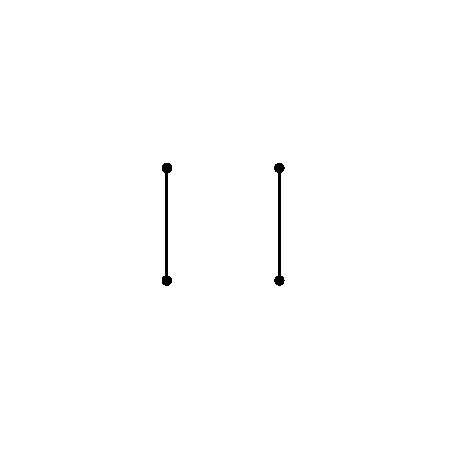
\includegraphics{Fig_5Z}
\end{figure}

\end{solution}

\ppart Since the Claim is false, there must be an logical mistake in the
following bogus proof.  Pinpoint the \emph{first} logical mistake
(unjustified step) in the proof.

\begin{bogusproof}
  We prove the Claim above by induction.  Let $P(n)$ be the proposition
  that if every vertex in an $n$-vertex graph has positive degree, then
  the graph is connected.

\textbf{Base cases}: ($n \leq 2$).  In a graph with 1 vertex, that vertex
cannot have positive degree, so $P(1)$ holds vacuously.

$P(2)$ holds because there is only one graph with two vertices of positive
degree, namely, the graph with an edge between the vertices, and this
graph is connected.

\textbf{Inductive step}: We must show that $P(n)$ implies
$P(n+1)$ for all $n \geq 2$.  Consider an $n$-vertex graph in which every
vertex has positive degree.  By the assumption $P(n)$, this graph is
connected; that is, there is a path between every pair of vertices.  Now
we add one more vertex $x$ to obtain an $(n+1)$-vertex graph:

\begin{figure}[h]\redrawn
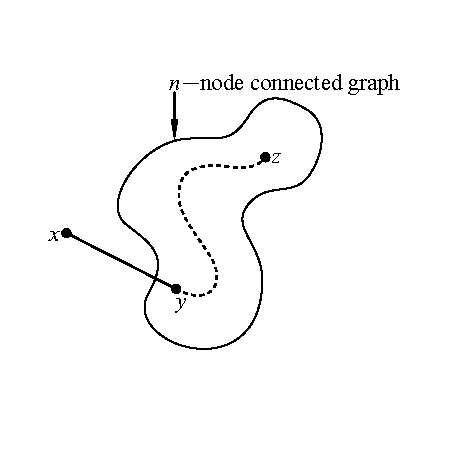
\includegraphics{false-connect-pic}
\end{figure}

All that remains is to check that there is a path from $x$ to every other
vertex $z$.  Since $x$ has positive degree, there is an edge from $x$ to
some other vertex, $y$.  Thus, we can obtain a path from $x$ to $z$
by going from $x$ to $y$ and then following the path from $y$ to $z$.  This
proves $P(n+1)$.

By the principle of induction, $P(n)$ is true for all $n \geq 0$, which
proves the Claim.

\end{bogusproof}

\begin{solution}
This one is tricky: the proof is actually a good proof of
something else.  The first error in the proof is only in the final
statement of the inductive step: ``This proves $P(n+1)$''.

The issue is that to prove $P(n+1)$, \emph{every} $(n+1)$-vertex
positive-degree graph must be shown to be connected.  But the proof
doesn't show this.  Instead, it shows that every $(n+1)$-vertex
positive-degree graph \emph{that can be built up by adding a vertex of
positive degree to an $n$-vertex connected graph}, is connected.

The problem is that \emph{not every} $(n+1)$-vertex positive-degree graph
can be built up in this way.  The counterexample above illustrates this:
there is no way to build that 4-vertex positive-degree graph from a
3-vertex positive-degree graph.

More generally, this is an example of ``buildup error''.  This error
arises from a faulty assumption that every size $n+1$ graph with some
property can be ``built up'' in some particular way from a size $n$ graph
with the same property.  (This assumption is correct for some properties,
but incorrect for others--- such as the one in the argument above.)

One way to avoid an accidental build-up error is to use a ``shrink
down, grow back'' process in the inductive step: start with a size
$n+1$ graph, remove a vertex (or edge), apply the inductive hypothesis
$P(n)$ to the smaller graph, and then add back the vertex (or edge)
and argue that $P(n+1)$ holds.  Let's see what would have happened if
we'd tried to prove the claim above by this method:

\noindent \textit{Inductive step:} We must show that $P(n)$ implies
$P(n+1)$ for all $n \geq 1$.  Consider an $(n+1)$-vertex graph $G$ in
which every vertex has degree at least 1.  Remove an arbitrary vertex
$v$, leaving an $n$-vertex graph $G'$ in which every vertex has
degree... uh-oh!

The reduced graph $G'$ might contain a vertex of degree 0, making the
inductive hypothesis $P(n)$ inapplicable!  We are stuck--- and
properly so, since the claim is false!
\end{solution}

\eparts
\end{problem}

%%%%%%%%%%%%%%%%%%%%%%%%%%%%%%%%%%%%%%%%%%%%%%%%%%%%%%%%%%%%%%%%%%%%%
% Problem ends here
%%%%%%%%%%%%%%%%%%%%%%%%%%%%%%%%%%%%%%%%%%%%%%%%%%%%%%%%%%%%%%%%%%%%%

\endinput
